\begin{frame}
	\frametitle{caso di studio: Reid [2011]}
	\framesubtitle{rete transazioni $\mathcal{T}$}
	
	% IDEA: partire da un'informazione pubblica, la blockchain, per associare
	% transazioni agli utenti
	
	% vertice == transazione t
	% arco diretto == flusso di BTC da un output di t a un input di t'
	
	% non è complesso costruire la rete: sono tutti dati pubblici
	% sono omesse transazioni non collegate ad altre transazioni, i.e. coinbase o fees non riscosse
	
	% il grafo è sicuramente un DAG; una transazione non può chiudersi su sè stessa!!!
	\begin{figure}[H]
	 	\begin{center}
			 \begin{tabular}{c @{\hspace{1em}} c}
				 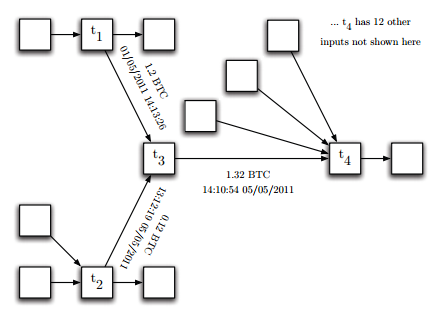
\includegraphics[height=6 cm]{images/anon_1.png}
			 \end{tabular}
		 \end{center}
 	\end{figure}

\end{frame}

\begin{frame}
	\frametitle{caso di studio: Reid [2011]}
	\framesubtitle{rete utenti imperfetta $\tilde{\mathcal{U}}$ }

	% occorre fare preprocessing per costruire la rete utenti

	% non sappiamo ancora chi siano gli utenti: ma come ammesso dallo stesso Satoshi, è estremamente probabile che
	% in una transazione con più di un input, tutte le chiavi {pk}_input appartengano allo stesso soggetto 
	% vertice diamante == chiave pubblica pk
	% adiacenza tra diamanti == supposizione di medesima proprietà
	% arco diretto == flusso di BTC da una pk a pk'
	
	% abbiamo iniziato ad accomunare delle chiavi pubbliche, ma possiam far di
	% più..

	\begin{figure}[H]
	 	\begin{center}
			 \begin{tabular}{c @{\hspace{1em}} c}
				 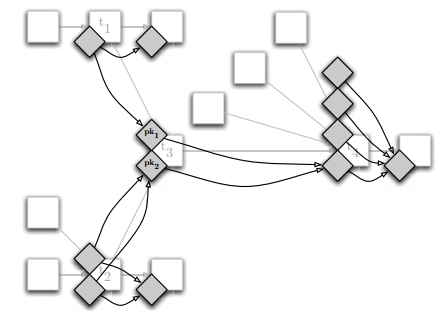
\includegraphics[height=6 cm]{images/anon_2.png}
			 \end{tabular}
		 \end{center}
 	\end{figure}
 	

\end{frame}

\begin{frame}
	\frametitle{caso di studio: Reid [2011]}
	\framesubtitle{rete utenti $\mathcal{U}$, rete ancella $\mathcal{A}$}
	
	%	vertice ancella == chiave pubblica 
	%	arco indiretto == paio di chiavi pubbliche in input a una stessa transazione
	% una rete ancella è qualcosa in più di una clique. 
	% 	diametro 4 -> almeno 2 pk dello stesso utente sono connesse indirettamente via 3 transazioni
	
	% IMP nel disegno è graficata un'ancella con ANCHE pks ESTERNE rispetto al sottoesempio
	% in particolare essendo dim(ancella u1)=16 => 
	
	% ogni componento connesso MASSIMALE costituisce un utente -> macrovertice cerchio
	
	% macrovertice cerchio == utente fisico
	% arco diretto == flusso di BTC da un utente a un altro
	
	% U, a differenza di T, non è più un DAG, ma può avere multiarchi e cicli 
	
	\begin{figure}[H]
	 	\begin{center}
			 \begin{tabular}{c @{\hspace{1em}} c}
				 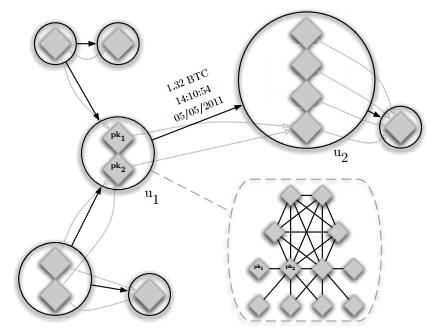
\includegraphics[height=6 cm]{images/anon_3.png}
			 \end{tabular}
		 \end{center}
 	\end{figure}

\end{frame}

\begin{frame}
	\frametitle{caso di studio: Reid [2011]}
	\framesubtitle{integrazione con informazioni esterne}
	
	% SAY forums, tweets
	
	\begin{itemize}
		\item dimensione $\propto |\{K_{PB}\}|$ utente
		\item colore $\propto$ \bitcoinA \;scambiati
	\end{itemize} 
	
	
	\begin{figure}[H]
	 	\begin{center}
			 \begin{tabular}{c @{\hspace{1em}} c}
				 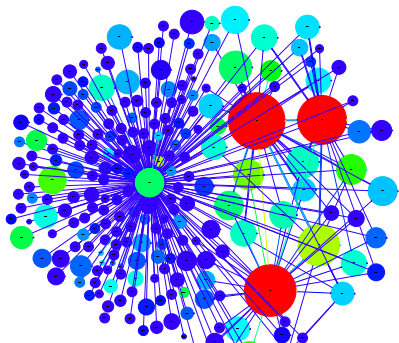
\includegraphics[height=6 cm]{images/anon_4.png}
			 \end{tabular}
		 \end{center}
 	\end{figure}

\end{frame}